\PassOptionsToPackage{unicode=true}{hyperref} % options for packages loaded elsewhere
\PassOptionsToPackage{hyphens}{url}
%
\documentclass[]{article}
\usepackage{lmodern}
\usepackage{amssymb,amsmath}
\usepackage{ifxetex,ifluatex}
\usepackage{fixltx2e} % provides \textsubscript
\ifnum 0\ifxetex 1\fi\ifluatex 1\fi=0 % if pdftex
  \usepackage[T1]{fontenc}
  \usepackage[utf8]{inputenc}
  \usepackage{textcomp} % provides euro and other symbols
\else % if luatex or xelatex
  \usepackage{unicode-math}
  \defaultfontfeatures{Ligatures=TeX,Scale=MatchLowercase}
\fi
% use upquote if available, for straight quotes in verbatim environments
\IfFileExists{upquote.sty}{\usepackage{upquote}}{}
% use microtype if available
\IfFileExists{microtype.sty}{%
\usepackage[]{microtype}
\UseMicrotypeSet[protrusion]{basicmath} % disable protrusion for tt fonts
}{}
\IfFileExists{parskip.sty}{%
\usepackage{parskip}
}{% else
\setlength{\parindent}{0pt}
\setlength{\parskip}{6pt plus 2pt minus 1pt}
}
\usepackage{hyperref}
\hypersetup{
            pdftitle={Regression Models: Assignment 2},
            pdfauthor={Daniel Alonso},
            pdfborder={0 0 0},
            breaklinks=true}
\urlstyle{same}  % don't use monospace font for urls
\usepackage[margin=1in]{geometry}
\usepackage{color}
\usepackage{fancyvrb}
\newcommand{\VerbBar}{|}
\newcommand{\VERB}{\Verb[commandchars=\\\{\}]}
\DefineVerbatimEnvironment{Highlighting}{Verbatim}{commandchars=\\\{\}}
% Add ',fontsize=\small' for more characters per line
\usepackage{framed}
\definecolor{shadecolor}{RGB}{248,248,248}
\newenvironment{Shaded}{\begin{snugshade}}{\end{snugshade}}
\newcommand{\AlertTok}[1]{\textcolor[rgb]{0.94,0.16,0.16}{#1}}
\newcommand{\AnnotationTok}[1]{\textcolor[rgb]{0.56,0.35,0.01}{\textbf{\textit{#1}}}}
\newcommand{\AttributeTok}[1]{\textcolor[rgb]{0.77,0.63,0.00}{#1}}
\newcommand{\BaseNTok}[1]{\textcolor[rgb]{0.00,0.00,0.81}{#1}}
\newcommand{\BuiltInTok}[1]{#1}
\newcommand{\CharTok}[1]{\textcolor[rgb]{0.31,0.60,0.02}{#1}}
\newcommand{\CommentTok}[1]{\textcolor[rgb]{0.56,0.35,0.01}{\textit{#1}}}
\newcommand{\CommentVarTok}[1]{\textcolor[rgb]{0.56,0.35,0.01}{\textbf{\textit{#1}}}}
\newcommand{\ConstantTok}[1]{\textcolor[rgb]{0.00,0.00,0.00}{#1}}
\newcommand{\ControlFlowTok}[1]{\textcolor[rgb]{0.13,0.29,0.53}{\textbf{#1}}}
\newcommand{\DataTypeTok}[1]{\textcolor[rgb]{0.13,0.29,0.53}{#1}}
\newcommand{\DecValTok}[1]{\textcolor[rgb]{0.00,0.00,0.81}{#1}}
\newcommand{\DocumentationTok}[1]{\textcolor[rgb]{0.56,0.35,0.01}{\textbf{\textit{#1}}}}
\newcommand{\ErrorTok}[1]{\textcolor[rgb]{0.64,0.00,0.00}{\textbf{#1}}}
\newcommand{\ExtensionTok}[1]{#1}
\newcommand{\FloatTok}[1]{\textcolor[rgb]{0.00,0.00,0.81}{#1}}
\newcommand{\FunctionTok}[1]{\textcolor[rgb]{0.00,0.00,0.00}{#1}}
\newcommand{\ImportTok}[1]{#1}
\newcommand{\InformationTok}[1]{\textcolor[rgb]{0.56,0.35,0.01}{\textbf{\textit{#1}}}}
\newcommand{\KeywordTok}[1]{\textcolor[rgb]{0.13,0.29,0.53}{\textbf{#1}}}
\newcommand{\NormalTok}[1]{#1}
\newcommand{\OperatorTok}[1]{\textcolor[rgb]{0.81,0.36,0.00}{\textbf{#1}}}
\newcommand{\OtherTok}[1]{\textcolor[rgb]{0.56,0.35,0.01}{#1}}
\newcommand{\PreprocessorTok}[1]{\textcolor[rgb]{0.56,0.35,0.01}{\textit{#1}}}
\newcommand{\RegionMarkerTok}[1]{#1}
\newcommand{\SpecialCharTok}[1]{\textcolor[rgb]{0.00,0.00,0.00}{#1}}
\newcommand{\SpecialStringTok}[1]{\textcolor[rgb]{0.31,0.60,0.02}{#1}}
\newcommand{\StringTok}[1]{\textcolor[rgb]{0.31,0.60,0.02}{#1}}
\newcommand{\VariableTok}[1]{\textcolor[rgb]{0.00,0.00,0.00}{#1}}
\newcommand{\VerbatimStringTok}[1]{\textcolor[rgb]{0.31,0.60,0.02}{#1}}
\newcommand{\WarningTok}[1]{\textcolor[rgb]{0.56,0.35,0.01}{\textbf{\textit{#1}}}}
\usepackage{graphicx,grffile}
\makeatletter
\def\maxwidth{\ifdim\Gin@nat@width>\linewidth\linewidth\else\Gin@nat@width\fi}
\def\maxheight{\ifdim\Gin@nat@height>\textheight\textheight\else\Gin@nat@height\fi}
\makeatother
% Scale images if necessary, so that they will not overflow the page
% margins by default, and it is still possible to overwrite the defaults
% using explicit options in \includegraphics[width, height, ...]{}
\setkeys{Gin}{width=\maxwidth,height=\maxheight,keepaspectratio}
\setlength{\emergencystretch}{3em}  % prevent overfull lines
\providecommand{\tightlist}{%
  \setlength{\itemsep}{0pt}\setlength{\parskip}{0pt}}
\setcounter{secnumdepth}{0}
% Redefines (sub)paragraphs to behave more like sections
\ifx\paragraph\undefined\else
\let\oldparagraph\paragraph
\renewcommand{\paragraph}[1]{\oldparagraph{#1}\mbox{}}
\fi
\ifx\subparagraph\undefined\else
\let\oldsubparagraph\subparagraph
\renewcommand{\subparagraph}[1]{\oldsubparagraph{#1}\mbox{}}
\fi

% set default figure placement to htbp
\makeatletter
\def\fps@figure{htbp}
\makeatother


\title{Regression Models: Assignment 2}
\author{Daniel Alonso}
\date{January 11th, 2020}

\begin{document}
\maketitle

\hypertarget{installing-libraries-used}{%
\subsection{Installing libraries used}\label{installing-libraries-used}}

\begin{Shaded}
\begin{Highlighting}[]
\NormalTok{packages =}\StringTok{ }\KeywordTok{c}\NormalTok{(}\StringTok{"dplyr"}\NormalTok{,}\StringTok{"MuMIn"}\NormalTok{,}\StringTok{"MASS"}\NormalTok{,}\StringTok{"leaps"}\NormalTok{,}\StringTok{"glmnet"}\NormalTok{,}\StringTok{"car"}\NormalTok{,}\StringTok{"stringr"}\NormalTok{,}\StringTok{"ResourceSelection"}
             \StringTok{"boot"}\NormalTok{,}\StringTok{"statmod"}\NormalTok{,}\StringTok{"Epi"}\NormalTok{, }\StringTok{"Metrics"}\NormalTok{, }\StringTok{"caret"}\NormalTok{, }\StringTok{"ggplot2"}\NormalTok{, }\StringTok{"multcomp"}\NormalTok{, }\StringTok{"combinat"}\NormalTok{)}
\ControlFlowTok{for}\NormalTok{ (package }\ControlFlowTok{in}\NormalTok{ packages) \{}
    \KeywordTok{install.packages}\NormalTok{(package)}
\NormalTok{\}}
\end{Highlighting}
\end{Shaded}

\hypertarget{importing-libraries}{%
\subsection{Importing libraries}\label{importing-libraries}}

\begin{Shaded}
\begin{Highlighting}[]
\KeywordTok{library}\NormalTok{(dplyr)}
\KeywordTok{library}\NormalTok{(MuMIn)}
\KeywordTok{library}\NormalTok{(MASS)}
\KeywordTok{library}\NormalTok{(leaps)}
\KeywordTok{library}\NormalTok{(glmnet)}
\KeywordTok{library}\NormalTok{(car)}
\KeywordTok{library}\NormalTok{(stringr)}
\KeywordTok{library}\NormalTok{(ResourceSelection)}
\KeywordTok{library}\NormalTok{(boot)}
\KeywordTok{library}\NormalTok{(statmod)}
\KeywordTok{library}\NormalTok{(Epi)}
\KeywordTok{library}\NormalTok{(Metrics)}
\KeywordTok{library}\NormalTok{(caret)}
\KeywordTok{library}\NormalTok{(ggplot2)}
\KeywordTok{library}\NormalTok{(multcomp)}
\KeywordTok{library}\NormalTok{(combinat)}
\end{Highlighting}
\end{Shaded}

\newpage

\hypertarget{exercise-1}{%
\subsection{Exercise 1}\label{exercise-1}}

\hypertarget{model-and-parameter-interpretation}{%
\subsubsection{Model and parameter
interpretation}\label{model-and-parameter-interpretation}}

\emph{Y} = Binary variable representing whether the customer will buy a
car or not \emph{income} = annual family income

Therefore we model the response as:

\(\eta = \beta_{0} + \beta_{1} X + \epsilon\)

And our values will be:

\(\eta = e^{-1.98079} + X e^{0.04342} + \epsilon\)

Where \(X\) is the annual family income.

The odds increase by \(e^{\beta_{1}} = 1.044376\) if the predictor is
increased by one unit.

\hypertarget{ci-for-the-probability-that-a-family-with-annual-income-of-60-thousand-dollars-will-purchase-a-new-car-next-year.}{%
\subsubsection{95\%-CI for the probability that a family with annual
income of 60 thousand dollars will purchase a new car next
year.}\label{ci-for-the-probability-that-a-family-with-annual-income-of-60-thousand-dollars-will-purchase-a-new-car-next-year.}}

We calculate the asymptotic \((1 - \alpha)\%\) confidence interval:

\(\hat{\beta_{j}} \pm z_{\frac{\alpha}{2}} S.E. (\hat{\beta_{j}})\)

With our values we get:

\begin{Shaded}
\begin{Highlighting}[]
\CommentTok{# defining a p function for prob}
\NormalTok{p =}\StringTok{ }\ControlFlowTok{function}\NormalTok{(eta) (}\KeywordTok{exp}\NormalTok{(eta)}\OperatorTok{/}\NormalTok{(}\KeywordTok{exp}\NormalTok{(eta)}\OperatorTok{+}\DecValTok{1}\NormalTok{))}

\CommentTok{# CI-Z}
\NormalTok{z_}\DecValTok{95}\NormalTok{ <-}\StringTok{ }\KeywordTok{qnorm}\NormalTok{(}\FloatTok{0.975}\NormalTok{)}

\CommentTok{# CI calculation}
\KeywordTok{p}\NormalTok{(}\OperatorTok{-}\FloatTok{1.98079} \OperatorTok{+}\StringTok{ }\NormalTok{z_}\DecValTok{95}\OperatorTok{*}\FloatTok{0.85720} \OperatorTok{+}\StringTok{ }\FloatTok{0.04342}\OperatorTok{*}\DecValTok{60} \OperatorTok{+}\StringTok{ }\NormalTok{z_}\DecValTok{95}\OperatorTok{*}\FloatTok{0.02011}\NormalTok{)}
\CommentTok{#> [1] 0.9124486}
\KeywordTok{p}\NormalTok{(}\OperatorTok{-}\FloatTok{1.98079} \OperatorTok{-}\StringTok{ }\NormalTok{z_}\DecValTok{95}\OperatorTok{*}\FloatTok{0.85720} \OperatorTok{+}\StringTok{ }\FloatTok{0.04342}\OperatorTok{*}\DecValTok{60} \OperatorTok{-}\StringTok{ }\NormalTok{z_}\DecValTok{95}\OperatorTok{*}\FloatTok{0.02011}\NormalTok{)}
\CommentTok{#> [1] 0.2506618}
\end{Highlighting}
\end{Shaded}

\(0.2506618 \leq p_{60k} \leq 0.9124486\)

\hypertarget{grouping-into-6-levels-of-income-what-test-is-used-and-what-are-the-df-of-the-test-statistic}{%
\subsubsection{Grouping into 6 levels of income, what test is used and
what are the DF of the test
statistic}\label{grouping-into-6-levels-of-income-what-test-is-used-and-what-are-the-df-of-the-test-statistic}}

The appropriate test for this would be the Hosmer-Lemeshow test with
\(G=6\) (corresponding to 6 groups).

The DF of the test statistic for a Hosmer-Lemeshow test is \(DF=G-2\),
therefore, \(DF = 4\)

\hypertarget{exercise-2}{%
\subsection{Exercise 2}\label{exercise-2}}

\hypertarget{importing-and-manipulating-the-dataset}{%
\subsubsection{Importing and manipulating the
dataset}\label{importing-and-manipulating-the-dataset}}

\begin{Shaded}
\begin{Highlighting}[]
\NormalTok{cols <-}\StringTok{ }\KeywordTok{c}\NormalTok{(}\StringTok{"age"}\NormalTok{,}\StringTok{"lwt"}\NormalTok{,}\StringTok{"race"}\NormalTok{,}\StringTok{"smoke"}\NormalTok{)}
\NormalTok{birthwt <-}\StringTok{ }\NormalTok{MASS}\OperatorTok{::}\NormalTok{birthwt }\OperatorTok\StringTok{ }\NormalTok{dplyr}\OperatorTok{::}\KeywordTok{select}\NormalTok{(}\KeywordTok{c}\NormalTok{(}\StringTok{"low"}\NormalTok{,cols))}
\end{Highlighting}
\end{Shaded}

For race we should use a dummy variable per race:

\begin{Shaded}
\begin{Highlighting}[]
\NormalTok{birthwt}\OperatorTok{$}\NormalTok{white <-}\StringTok{ }\KeywordTok{ifelse}\NormalTok{(birthwt}\OperatorTok{$}\NormalTok{race }\OperatorTok{==}\StringTok{ }\DecValTok{1}\NormalTok{, }\DecValTok{1}\NormalTok{, }\DecValTok{0}\NormalTok{)}
\NormalTok{birthwt}\OperatorTok{$}\NormalTok{black <-}\StringTok{ }\KeywordTok{ifelse}\NormalTok{(birthwt}\OperatorTok{$}\NormalTok{race }\OperatorTok{==}\StringTok{ }\DecValTok{2}\NormalTok{, }\DecValTok{1}\NormalTok{, }\DecValTok{0}\NormalTok{)}
\NormalTok{birthwt}\OperatorTok{$}\NormalTok{other <-}\StringTok{ }\KeywordTok{ifelse}\NormalTok{(birthwt}\OperatorTok{$}\NormalTok{race }\OperatorTok{==}\StringTok{ }\DecValTok{3}\NormalTok{, }\DecValTok{1}\NormalTok{, }\DecValTok{0}\NormalTok{)}
\NormalTok{cols <-}\StringTok{ }\KeywordTok{c}\NormalTok{(}\StringTok{"age"}\NormalTok{, }\StringTok{"lwt"}\NormalTok{, }\StringTok{"smoke"}\NormalTok{, }\StringTok{"white"}\NormalTok{, }\StringTok{"black"}\NormalTok{, }\StringTok{"other"}\NormalTok{)}
\NormalTok{birthwt <-}\StringTok{ }\NormalTok{birthwt }\OperatorTok\StringTok{ }\NormalTok{dplyr}\OperatorTok{::}\KeywordTok{select}\NormalTok{(}\KeywordTok{c}\NormalTok{(}\StringTok{"low"}\NormalTok{,cols))}
\end{Highlighting}
\end{Shaded}

\hypertarget{model-fitting-and-selection}{%
\subsubsection{Model fitting and
selection}\label{model-fitting-and-selection}}

\begin{Shaded}
\begin{Highlighting}[]
\NormalTok{FM <-}\StringTok{ }\KeywordTok{glm}\NormalTok{(low }\OperatorTok{~}\StringTok{ }\NormalTok{., }\DataTypeTok{data=}\NormalTok{birthwt, }\DataTypeTok{family=}\NormalTok{binomial)}
\NormalTok{staic <-}\StringTok{ }\KeywordTok{stepAIC}\NormalTok{(FM, }\KeywordTok{list}\NormalTok{(}\DataTypeTok{upper=}\OperatorTok{~}\NormalTok{age}\OperatorTok{*}\NormalTok{lwt}\OperatorTok{*}\NormalTok{smoke}\OperatorTok{*}\NormalTok{white}\OperatorTok{*}\NormalTok{black}\OperatorTok{*}\NormalTok{other, }\DataTypeTok{lower=} \OperatorTok{~}\DecValTok{1}\NormalTok{))}
\CommentTok{#> Start:  AIC=226.58}
\CommentTok{#> low ~ age + lwt + smoke + white + black + other}
\CommentTok{#> }
\CommentTok{#> }
\CommentTok{#> Step:  AIC=226.58}
\CommentTok{#> low ~ age + lwt + smoke + white + black}
\CommentTok{#> }
\CommentTok{#>               Df Deviance    AIC}
\CommentTok{#> - black        1   214.88 224.88}
\CommentTok{#> - age          1   215.01 225.01}
\CommentTok{#> <none>             214.58 226.58}
\CommentTok{#> + smoke:white  1   213.16 227.16}
\CommentTok{#> + lwt:smoke    1   213.66 227.66}
\CommentTok{#> + age:black    1   214.05 228.05}
\CommentTok{#> + lwt:black    1   214.05 228.05}
\CommentTok{#> + age:smoke    1   214.25 228.25}
\CommentTok{#> + lwt:white    1   214.45 228.45}
\CommentTok{#> + smoke:black  1   214.49 228.49}
\CommentTok{#> + age:lwt      1   214.55 228.55}
\CommentTok{#> + age:white    1   214.56 228.56}
\CommentTok{#> - lwt          1   218.86 228.86}
\CommentTok{#> - white        1   219.89 229.89}
\CommentTok{#> - smoke        1   222.66 232.66}
\CommentTok{#> }
\CommentTok{#> Step:  AIC=224.88}
\CommentTok{#> low ~ age + lwt + smoke + white}
\CommentTok{#> }
\CommentTok{#>               Df Deviance    AIC}
\CommentTok{#> - age          1   215.38 223.38}
\CommentTok{#> <none>             214.88 224.88}
\CommentTok{#> + smoke:white  1   213.67 225.67}
\CommentTok{#> + lwt:smoke    1   214.12 226.12}
\CommentTok{#> + age:smoke    1   214.47 226.47}
\CommentTok{#> + black        1   214.58 226.58}
\CommentTok{#> + other        1   214.58 226.58}
\CommentTok{#> + lwt:white    1   214.83 226.83}
\CommentTok{#> + age:lwt      1   214.83 226.83}
\CommentTok{#> - lwt          1   218.87 226.87}
\CommentTok{#> + age:white    1   214.87 226.87}
\CommentTok{#> - white        1   222.88 230.88}
\CommentTok{#> - smoke        1   223.85 231.85}
\CommentTok{#> }
\CommentTok{#> Step:  AIC=223.38}
\CommentTok{#> low ~ lwt + smoke + white}
\CommentTok{#> }
\CommentTok{#>               Df Deviance    AIC}
\CommentTok{#> <none>             215.38 223.38}
\CommentTok{#> + smoke:white  1   213.94 223.94}
\CommentTok{#> + lwt:smoke    1   214.62 224.62}
\CommentTok{#> + age          1   214.88 224.88}
\CommentTok{#> + black        1   215.01 225.01}
\CommentTok{#> + other        1   215.01 225.01}
\CommentTok{#> + lwt:white    1   215.31 225.31}
\CommentTok{#> - lwt          1   219.98 225.98}
\CommentTok{#> - white        1   224.34 230.34}
\CommentTok{#> - smoke        1   224.65 230.65}
\end{Highlighting}
\end{Shaded}

Using stepAIC we can see all the combinations classified by AIC. The
model with the lowest AIC is the model that uses \emph{lwt},
\emph{smoke} and \emph{white} and drops the \emph{age}, \emph{black} and
\emph{other} variables.

We can see the interactions between the variable selected and age are
not particularly significant and don't seem to affect the model enough
to consider them, in fact, the AIC is improved when these are not
present.

We can see that in general, dropping the \emph{age} variable yields a
better result:

\begin{Shaded}
\begin{Highlighting}[]
\NormalTok{staic}\OperatorTok{$}\NormalTok{anova}
\CommentTok{#> Stepwise Model Path }
\CommentTok{#> Analysis of Deviance Table}
\CommentTok{#> }
\CommentTok{#> Initial Model:}
\CommentTok{#> low ~ age + lwt + smoke + white + black + other}
\CommentTok{#> }
\CommentTok{#> Final Model:}
\CommentTok{#> low ~ lwt + smoke + white}
\CommentTok{#> }
\CommentTok{#> }
\CommentTok{#>      Step Df  Deviance Resid. Df Resid. Dev      AIC}
\CommentTok{#> 1                            183   214.5772 226.5772}
\CommentTok{#> 2 - other  0 0.0000000       183   214.5772 226.5772}
\CommentTok{#> 3 - black  1 0.2991850       184   214.8764 224.8764}
\CommentTok{#> 4   - age  1 0.5068236       185   215.3832 223.3832}
\end{Highlighting}
\end{Shaded}

\begin{Shaded}
\begin{Highlighting}[]
\KeywordTok{options}\NormalTok{(}\DataTypeTok{na.action=}\NormalTok{na.fail)}
\NormalTok{MuMIn}\OperatorTok{::}\KeywordTok{dredge}\NormalTok{(FM)}
\end{Highlighting}
\end{Shaded}

Using dredge also tells us the same as stepAIC, where the best model is
the one at the top (as they are ranked by AIC already).

\begin{Shaded}
\begin{Highlighting}[]
\KeywordTok{anova}\NormalTok{(FM, staic, }\DataTypeTok{test=}\StringTok{"Chisq"}\NormalTok{)}\OperatorTok{$}\StringTok{"Pr(>Chi)"}\NormalTok{[}\DecValTok{2}\NormalTok{]}
\CommentTok{#> [1] 0.6683092}
\end{Highlighting}
\end{Shaded}

Performing a likelihood ratio test yields a good, high p-val of 0.668 so
we pick the reduced model.

\hypertarget{hosmer-lemeshow-test}{%
\subsubsection{Hosmer-Lemeshow test}\label{hosmer-lemeshow-test}}

\begin{Shaded}
\begin{Highlighting}[]
\KeywordTok{hoslem.test}\NormalTok{(birthwt}\OperatorTok{$}\NormalTok{low, }\KeywordTok{predict}\NormalTok{(staic, }\DataTypeTok{type=}\StringTok{"response"}\NormalTok{))}
\CommentTok{#> }
\CommentTok{#>  Hosmer and Lemeshow goodness of fit (GOF) test}
\CommentTok{#> }
\CommentTok{#> data:  birthwt$low, predict(staic, type = "response")}
\CommentTok{#> X-squared = 9.0869, df = 8, p-value = 0.335}
\end{Highlighting}
\end{Shaded}

We have a large p-value of 0.335 which indicates that our goodness of
fit is most likely okay.

\newpage

\hypertarget{residual-plots-and-model-assumptions}{%
\subsubsection{Residual plots and model
assumptions}\label{residual-plots-and-model-assumptions}}

\begin{Shaded}
\begin{Highlighting}[]
\KeywordTok{glm.diag.plots}\NormalTok{(staic)}
\end{Highlighting}
\end{Shaded}

\includegraphics{./figures/unnamed-chunk-12-1.pdf}

As we have 2 sets of points for the Residuals vs Linear predictor and
the Quantiles of standard normal vs Ordered deviance residuals, we can't
properly interpret these.

For the cook's distance we can see there is a few slightly high leverage
points . However, it is not significant as other than this there's no
points present in the top right quadrant of the plot.

\newpage

\begin{Shaded}
\begin{Highlighting}[]
\KeywordTok{par}\NormalTok{(}\DataTypeTok{mfrow=}\KeywordTok{c}\NormalTok{(}\DecValTok{2}\NormalTok{,}\DecValTok{1}\NormalTok{))}
\KeywordTok{plot}\NormalTok{(birthwt}\OperatorTok{$}\NormalTok{lwt, }\KeywordTok{qres.binom}\NormalTok{(staic), }\DataTypeTok{xlab=}\StringTok{"lwt"}\NormalTok{, }\DataTypeTok{ylab=}\StringTok{"Quantile residuals"}\NormalTok{)}
\KeywordTok{qqnorm}\NormalTok{(}\KeywordTok{qres.binom}\NormalTok{(staic))}
\end{Highlighting}
\end{Shaded}

\includegraphics{./figures/unnamed-chunk-13-1.pdf}

We decide not to plot the \emph{race} or \emph{smoke} variables given
that, even though they're in the model, they're categorical variables.

For our \emph{lwt} residual plot, everything seems to be okay, we see
that. In the normal QQ plot we see that the values decently fit a normal
distribution. This fits the normality assumption.

Our only continuous variable in the model (\emph{lwt}) seems to have
constant variance, therefore our model is homocedastic.

\newpage

\hypertarget{total-error-rate-of-the-model}{%
\subsubsection{Total error rate of the
model}\label{total-error-rate-of-the-model}}

\begin{Shaded}
\begin{Highlighting}[]
\NormalTok{Epi}\OperatorTok{::}\KeywordTok{ROC}\NormalTok{(}\DataTypeTok{form=}\NormalTok{low}\OperatorTok{~}\NormalTok{lwt}\OperatorTok{+}\NormalTok{white}\OperatorTok{+}\NormalTok{smoke , }\DataTypeTok{data=}\NormalTok{birthwt, }\DataTypeTok{plot=}\StringTok{"ROC"}\NormalTok{, }\DataTypeTok{lw=}\DecValTok{3}\NormalTok{, }\DataTypeTok{cex=}\FloatTok{1.5}\NormalTok{)}
\end{Highlighting}
\end{Shaded}

\includegraphics{./figures/unnamed-chunk-14-1.pdf}

The model has an AUC = 0.684 which corresponds to a decent but not
particularly good model, however, using this measure we can assert that
the model does have predictive capability.

We can see our cutoff point is also 0.253.

Our model has a very high sensitivity, however, a very low specificity,
therefore it also has a very high false negative rate. We could
comfortably assert that this is the achilles heel of our model, as it
still has a high accuracy for positives but a very low accuracy for
negatives.

It would also be appropriate to look at the MAE and MSE for our model.

\begin{Shaded}
\begin{Highlighting}[]
\NormalTok{Metrics}\OperatorTok{::}\KeywordTok{mae}\NormalTok{(birthwt}\OperatorTok{$}\NormalTok{low, }\KeywordTok{predict}\NormalTok{(staic, }\DataTypeTok{type=}\StringTok{"response"}\NormalTok{))}
\CommentTok{#> [1] 0.3893964}
\NormalTok{Metrics}\OperatorTok{::}\KeywordTok{mse}\NormalTok{(birthwt}\OperatorTok{$}\NormalTok{low, }\KeywordTok{predict}\NormalTok{(staic, }\DataTypeTok{type=}\StringTok{"response"}\NormalTok{))}
\CommentTok{#> [1] 0.1956847}
\end{Highlighting}
\end{Shaded}

We can see that they're both relatively low even though our model
doesn't perform amazingly.

\hypertarget{mothers-having-babies-with-low-birth-weight-vs-normal-birth-weight}{%
\subsubsection{Mothers having babies with low birth weight vs normal
birth
weight}\label{mothers-having-babies-with-low-birth-weight-vs-normal-birth-weight}}

First we will look at variable importance:

\begin{Shaded}
\begin{Highlighting}[]
\NormalTok{caret}\OperatorTok{::}\KeywordTok{varImp}\NormalTok{(staic)}
\CommentTok{#>        Overall}
\CommentTok{#> lwt   2.029237}
\CommentTok{#> smoke 2.962211}
\CommentTok{#> white 2.888260}
\end{Highlighting}
\end{Shaded}

We can see that the most important variable of the model is the
\emph{smoke} variable, followed by \emph{white} and then \emph{lwt}.

We select a subset of the original dataset which uses the model
prediction and we also select a subset of the original dataset using the
real classification. Both for normal birth weight babies and low birth
weight babies, in order to assess which elements are characteristic of
each group.

\begin{Shaded}
\begin{Highlighting}[]
\CommentTok{# model's prediction}
\NormalTok{pred <-}\StringTok{ }\KeywordTok{predict}\NormalTok{(staic, }\DataTypeTok{type=}\StringTok{"response"}\NormalTok{)}
\NormalTok{normal_birth_weight <-}\StringTok{ }\NormalTok{birthwt[pred}\OperatorTok{<}\FloatTok{0.253}\NormalTok{,]}
\NormalTok{low_birth_weight <-}\StringTok{ }\NormalTok{birthwt[pred}\OperatorTok{>}\FloatTok{0.253}\NormalTok{,]}

\CommentTok{# reality}
\NormalTok{real_lbw <-}\StringTok{ }\NormalTok{birthwt }\OperatorTok\StringTok{ }\NormalTok{dplyr}\OperatorTok{::}\KeywordTok{filter}\NormalTok{(low }\OperatorTok{==}\StringTok{ }\DecValTok{1}\NormalTok{)}
\NormalTok{real_nbw <-}\StringTok{ }\NormalTok{birthwt }\OperatorTok\StringTok{ }\NormalTok{dplyr}\OperatorTok{::}\KeywordTok{filter}\NormalTok{(low }\OperatorTok{==}\StringTok{ }\DecValTok{0}\NormalTok{)}
\end{Highlighting}
\end{Shaded}

\hypertarget{smoke-prevalence}{%
\paragraph{Smoke prevalence}\label{smoke-prevalence}}

\begin{Shaded}
\begin{Highlighting}[]
\KeywordTok{table}\NormalTok{(normal_birth_weight}\OperatorTok{$}\NormalTok{smoke)}
\CommentTok{#> }
\CommentTok{#>  0  1 }
\CommentTok{#> 53  7}
\end{Highlighting}
\end{Shaded}

We can see that as the model considers the variable smoke particularly
important for prediction, it seems to very strongly influence its
prediction of normal birth weight, therefore very effectively predicting
those with normal birth weight. And as we clearly know, smoking is a
high risk factor for birth issues like this. However, we can also notice
that non-smokers tend to give birth to normal weight babies.

\begin{Shaded}
\begin{Highlighting}[]
\KeywordTok{table}\NormalTok{(low_birth_weight}\OperatorTok{$}\NormalTok{smoke)}
\CommentTok{#> }
\CommentTok{#>  0  1 }
\CommentTok{#> 62 67}
\end{Highlighting}
\end{Shaded}

However, when comparing its prediction of low birth weight it falls
short, as not all low birth weight babies come from a mother that
smokes. The model fails about 60\% of the time.

In contrast to the reality:

\begin{Shaded}
\begin{Highlighting}[]
\KeywordTok{table}\NormalTok{(real_lbw}\OperatorTok{$}\NormalTok{smoke)}
\CommentTok{#> }
\CommentTok{#>  0  1 }
\CommentTok{#> 29 30}
\end{Highlighting}
\end{Shaded}

For low weight babies there's about a 50\% chance that the mother is a
smoker

\begin{Shaded}
\begin{Highlighting}[]
\KeywordTok{table}\NormalTok{(real_nbw}\OperatorTok{$}\NormalTok{smoke)}
\CommentTok{#> }
\CommentTok{#>  0  1 }
\CommentTok{#> 86 44}
\end{Highlighting}
\end{Shaded}

While it is significantly more probable that the mother is not a smoker
when the baby has a normal birth weight. We see that the amount of
non-smoker mothers represent about 66\% of the normal birth weight
subset.

\newpage

\hypertarget{age}{%
\paragraph{Age}\label{age}}

\begin{verbatim}
#> [1] "low birth weight: 22.3488372093023"
#> [1] "normal birth weight: 25.15"
\end{verbatim}

We can see that according to the model, the median age of mothers giving
birth to normal weight babies is \textasciitilde{}25.15 years old, while
the ones with low birth weight babies are \textasciitilde{}22.35 years
old.

In contrast to the reality though:

\begin{verbatim}
#> [1] "low birth weight: 22.3050847457627"
#> [1] "normal birth weight: 23.6615384615385"
\end{verbatim}

There doesn't seem to be a significant age difference
(\textasciitilde{}1 year).

\hypertarget{mothers-weight}{%
\paragraph{Mother's weight}\label{mothers-weight}}

\begin{Shaded}
\begin{Highlighting}[]
\KeywordTok{print}\NormalTok{(stringr}\OperatorTok{::}\KeywordTok{str_interp}\NormalTok{(}\StringTok{'low birth weight: $\{mean(low_birth_weight$lwt)\}'}\NormalTok{))}
\CommentTok{#> [1] "low birth weight: 119.015503875969"}
\KeywordTok{print}\NormalTok{(stringr}\OperatorTok{::}\KeywordTok{str_interp}\NormalTok{(}\StringTok{'normal birth weight: $\{mean(normal_birth_weight$lwt)\}'}\NormalTok{))}
\CommentTok{#> [1] "normal birth weight: 153.033333333333"}
\end{Highlighting}
\end{Shaded}

The mother's weight shows significant difference for the prediction,
where normal birth weight mom's weight (on average) about 34 pounds
more.

\begin{Shaded}
\begin{Highlighting}[]
\KeywordTok{print}\NormalTok{(stringr}\OperatorTok{::}\KeywordTok{str_interp}\NormalTok{(}\StringTok{'low birth weight: $\{mean(real_lbw$lwt)\}'}\NormalTok{))}
\CommentTok{#> [1] "low birth weight: 122.135593220339"}
\KeywordTok{print}\NormalTok{(stringr}\OperatorTok{::}\KeywordTok{str_interp}\NormalTok{(}\StringTok{'normal birth weight: $\{mean(real_nbw$lwt)\}'}\NormalTok{))}
\CommentTok{#> [1] "normal birth weight: 133.3"}
\end{Highlighting}
\end{Shaded}

However, in reality, the difference is \textasciitilde{}11 pounds on
average for our dataset.

\hypertarget{mothers-race-binary-if-white}{%
\paragraph{Mother's race (binary if
white)}\label{mothers-race-binary-if-white}}

\begin{Shaded}
\begin{Highlighting}[]
\KeywordTok{table}\NormalTok{(low_birth_weight}\OperatorTok{$}\NormalTok{white)}
\CommentTok{#> }
\CommentTok{#>  0  1 }
\CommentTok{#> 83 46}
\end{Highlighting}
\end{Shaded}

The model is significantly biased towards the white race group where
most low birth weight babies come from non-white mothers (about 2x more
likely).

\begin{Shaded}
\begin{Highlighting}[]
\KeywordTok{table}\NormalTok{(normal_birth_weight}\OperatorTok{$}\NormalTok{white)}
\CommentTok{#> }
\CommentTok{#>  0  1 }
\CommentTok{#> 10 50}
\end{Highlighting}
\end{Shaded}

We also see that race group 1 has the highest representation among those
mothers with normal birth weight babies.

In contrast to the reality:

\begin{Shaded}
\begin{Highlighting}[]
\KeywordTok{table}\NormalTok{(real_lbw}\OperatorTok{$}\NormalTok{white)}
\CommentTok{#> }
\CommentTok{#>  0  1 }
\CommentTok{#> 36 23}
\end{Highlighting}
\end{Shaded}

We can see that in the real dataset, race doesn't quite seem to play the
role that the model portrays it to have in whether a baby has low birth
weight or not.

\begin{Shaded}
\begin{Highlighting}[]
\KeywordTok{table}\NormalTok{(real_lbw}\OperatorTok{$}\NormalTok{white)}
\CommentTok{#> }
\CommentTok{#>  0  1 }
\CommentTok{#> 36 23}
\KeywordTok{table}\NormalTok{(real_nbw}\OperatorTok{$}\NormalTok{white)}
\CommentTok{#> }
\CommentTok{#>  0  1 }
\CommentTok{#> 57 73}
\end{Highlighting}
\end{Shaded}

There's a clear overrepresentation of race group 1 in the normal birth
weight subset.

\hypertarget{what-characteristic-had-the-highest-impact}{%
\paragraph{What characteristic had the highest
impact?}\label{what-characteristic-had-the-highest-impact}}

Following the model's result, we can definitely say that whether the
mother was a smoker or not had the highest influence in its prediction,
followed by the race, where there was a huge overrepresentation of group
3 in the low birth weight group.

\hypertarget{exercise-3}{%
\subsection{Exercise 3}\label{exercise-3}}

\begin{Shaded}
\begin{Highlighting}[]
\NormalTok{health <-}\StringTok{ }\KeywordTok{read.table}\NormalTok{(}\StringTok{'../data/health.txt'}\NormalTok{, }\DataTypeTok{header=}\OtherTok{TRUE}\NormalTok{)}
\NormalTok{cols <-}\StringTok{ }\KeywordTok{c}\NormalTok{(}\StringTok{"g02"}\NormalTok{,}\StringTok{"sex"}\NormalTok{,}\StringTok{"weight"}\NormalTok{)}
\NormalTok{health <-}\StringTok{ }\NormalTok{health }\OperatorTok\StringTok{ }\NormalTok{dplyr}\OperatorTok{::}\KeywordTok{select}\NormalTok{(g02,sex,weight)}
\end{Highlighting}
\end{Shaded}

\begin{Shaded}
\begin{Highlighting}[]
\KeywordTok{mean}\NormalTok{(health[health}\OperatorTok{$}\NormalTok{sex}\OperatorTok{==}\DecValTok{1}\NormalTok{,]}\OperatorTok{$}\NormalTok{weight)}
\CommentTok{#> [1] 77.89171}
\KeywordTok{mean}\NormalTok{(health[health}\OperatorTok{$}\NormalTok{sex}\OperatorTok{==}\DecValTok{2}\NormalTok{,]}\OperatorTok{$}\NormalTok{weight)}
\CommentTok{#> [1] 61.18423}
\end{Highlighting}
\end{Shaded}

We will make the assumption that for the \emph{sex} column \emph{1 =
males} and \emph{2 = females}, as average weight for males is
(generally) higher for pretty much every country.

We will subtract 1 from the \emph{sex} column to make it a binary
variable with only 1s and 0s.

\begin{Shaded}
\begin{Highlighting}[]
\NormalTok{health}\OperatorTok{$}\NormalTok{sex <-}\StringTok{ }\NormalTok{health}\OperatorTok{$}\NormalTok{sex }\OperatorTok{-}\StringTok{ }\DecValTok{1}
\end{Highlighting}
\end{Shaded}

\begin{Shaded}
\begin{Highlighting}[]
\NormalTok{fm <-}\StringTok{ }\KeywordTok{glm}\NormalTok{(g02 }\OperatorTok{~}\StringTok{ }\NormalTok{sex}\OperatorTok{+}\NormalTok{weight}\OperatorTok{+}\NormalTok{sex}\OperatorTok{:}\NormalTok{weight, }\DataTypeTok{data=}\NormalTok{health, }\DataTypeTok{family=}\NormalTok{binomial)}
\NormalTok{model <-}\StringTok{ }\KeywordTok{glm}\NormalTok{(g02 }\OperatorTok{~}\StringTok{ }\NormalTok{sex}\OperatorTok{+}\NormalTok{weight, }\DataTypeTok{data=}\NormalTok{health, }\DataTypeTok{family=}\NormalTok{binomial)}
\KeywordTok{anova}\NormalTok{(fm, model, }\DataTypeTok{test=}\StringTok{"Chisq"}\NormalTok{)}
\CommentTok{#> Analysis of Deviance Table}
\CommentTok{#> }
\CommentTok{#> Model 1: g02 ~ sex + weight + sex:weight}
\CommentTok{#> Model 2: g02 ~ sex + weight}
\CommentTok{#>   Resid. Df Resid. Dev Df Deviance Pr(>Chi)    }
\CommentTok{#> 1      7353     7013.5                         }
\CommentTok{#> 2      7354     7042.3 -1  -28.858 7.79e-08 ***}
\CommentTok{#> ---}
\CommentTok{#> Signif. codes:  0 '***' 0.001 '**' 0.01 '*' 0.05 '.' 0.1 ' ' 1}
\end{Highlighting}
\end{Shaded}

The interaction between sex and weight is significant, therefore we will
include it in the model.

\newpage

\hypertarget{interpreting-the-coefficients-in-terms-of-the-or}{%
\subsubsection{Interpreting the coefficients in terms of the
OR}\label{interpreting-the-coefficients-in-terms-of-the-or}}

\(\eta = log(\frac{p}{1-p})\)

\(\eta = \beta_0 + \beta_1 x_1 + \beta_2 x_2 + \dots + \beta_k x_k\)

In terms of the odds:

\(Odds = e^{2.56152 + 1.236831 X_1 - 0.01171 X_2 - 0.028984 X_1 X_2}\)

Where \(X_1\) represents \emph{sex}, \(X_2\) represents \emph{weight}
and \(X_1 X_2\) represents \emph{sex:weight}.

For the odds ratio, we should highlight the differences between males
and females.

Therefore:

\(O_R = \frac{e^{2.56152 - 0.01171 X_2}}{e^{2.56152 + 1.236831 X_1 - 0.01171 X_2 - 0.028984 X_1 X_2}}\)

Where the numerator of the fraction corresponds to the odds for
\textbf{males} and the denominator corresponds to the odds for
\textbf{females}.

\hypertarget{plotting-predicted-probabilities-for-males-and-females}{%
\subsubsection{Plotting predicted probabilities for males and
females}\label{plotting-predicted-probabilities-for-males-and-females}}

\begin{Shaded}
\begin{Highlighting}[]
\NormalTok{health}\OperatorTok{$}\NormalTok{pred_prob <-}\StringTok{ }\KeywordTok{predict}\NormalTok{(fm, }\DataTypeTok{type=}\StringTok{'response'}\NormalTok{)}
\NormalTok{Sex <-}\StringTok{ }\KeywordTok{ifelse}\NormalTok{(health}\OperatorTok{$}\NormalTok{sex }\OperatorTok{==}\StringTok{ }\DecValTok{1}\NormalTok{, }\StringTok{"female"}\NormalTok{, }\StringTok{"male"}\NormalTok{)}
\KeywordTok{ggplot}\NormalTok{(}\DataTypeTok{data=}\NormalTok{health, }\KeywordTok{aes}\NormalTok{(}\DataTypeTok{color=}\NormalTok{Sex)) }\OperatorTok{+}\StringTok{ }\KeywordTok{geom_point}\NormalTok{(}\KeywordTok{aes}\NormalTok{(}\DataTypeTok{x=}\NormalTok{weight, }\DataTypeTok{y=}\NormalTok{pred_prob))}
\end{Highlighting}
\end{Shaded}

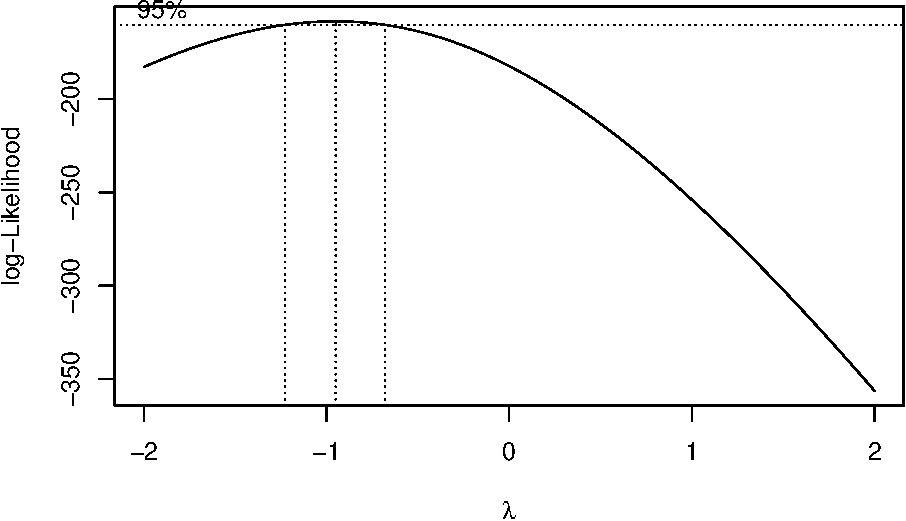
\includegraphics{./figures/unnamed-chunk-34-1.pdf}

We can see a trend here, men are significantly more likely to consider
themselves healthy. The model is also telling us that weight negatively
affects the probability to feel healthy in a significant way, however,
much more significantly on females than males.

Both men and women seem to consider weight an important factor in their
health perception. The lower usually tends to mean the better, however,
it's clear that being underweight isn't a healthy trait, but some people
might think otherwise.

\newpage

\hypertarget{relative-risk-and-odds-ratio-of-self-perceived-good-health-per-sex-for-a-75kg-person}{%
\subsubsection{Relative risk and odds ratio of self-perceived good
health per sex for a 75kg
person}\label{relative-risk-and-odds-ratio-of-self-perceived-good-health-per-sex-for-a-75kg-person}}

We predict for both males and females by specifying the \emph{sex=0}
(for males) and \emph{sex=1} (for females) and \emph{weight=75} for both
sexes.

\begin{Shaded}
\begin{Highlighting}[]
\NormalTok{males <-}\StringTok{ }\KeywordTok{predict}\NormalTok{(fm, }\DataTypeTok{newdata=}\KeywordTok{data.frame}\NormalTok{(}\DataTypeTok{sex=}\DecValTok{0}\NormalTok{,}\DataTypeTok{weight=}\DecValTok{75}\NormalTok{), }\DataTypeTok{type=}\StringTok{"response"}\NormalTok{)}
\NormalTok{females <-}\StringTok{ }\KeywordTok{predict}\NormalTok{(fm, }\DataTypeTok{newdata=}\KeywordTok{data.frame}\NormalTok{(}\DataTypeTok{sex=}\DecValTok{1}\NormalTok{,}\DataTypeTok{weight=}\DecValTok{75}\NormalTok{), }\DataTypeTok{type=}\StringTok{"response"}\NormalTok{)}
\end{Highlighting}
\end{Shaded}

We calculate the relative risk:

\begin{Shaded}
\begin{Highlighting}[]
\NormalTok{females}\OperatorTok{/}\NormalTok{males}
\CommentTok{#>         1 }
\CommentTok{#> 0.8043606}
\end{Highlighting}
\end{Shaded}

And the odds Ratio:

\begin{Shaded}
\begin{Highlighting}[]
\NormalTok{(females}\OperatorTok{/}\NormalTok{(}\DecValTok{1}\OperatorTok{-}\NormalTok{females))}\OperatorTok{/}\NormalTok{(males}\OperatorTok{/}\NormalTok{(}\DecValTok{1}\OperatorTok{-}\NormalTok{males))}
\CommentTok{#>         1 }
\CommentTok{#> 0.3918128}
\end{Highlighting}
\end{Shaded}

We can say that females are \emph{0.3918128} times less likely to have
self-perceived good health than males.

\hypertarget{estimated-expected-probability-of-self-perceived-good-health-of-females-of-70kg-and-110kg-with-ci}{%
\subsubsection{Estimated expected probability of self-perceived good
health of females of 70kg and 110kg with
CI}\label{estimated-expected-probability-of-self-perceived-good-health-of-females-of-70kg-and-110kg-with-ci}}

\hypertarget{females-of-70kg}{%
\paragraph{Females of 70kg}\label{females-of-70kg}}

\begin{Shaded}
\begin{Highlighting}[]
\KeywordTok{predict}\NormalTok{(fm, }\DataTypeTok{newdata=}\KeywordTok{data.frame}\NormalTok{(}\DataTypeTok{sex=}\DecValTok{1}\NormalTok{,}\DataTypeTok{weight=}\DecValTok{70}\NormalTok{), }\DataTypeTok{type=}\StringTok{"response"}\NormalTok{)}
\CommentTok{#>         1 }
\CommentTok{#> 0.7210275}
\end{Highlighting}
\end{Shaded}

The expected probability of self-perceived good health for 70kg females
is of \textasciitilde{}0.721.

\hypertarget{females-of-110kg}{%
\paragraph{Females of 110kg}\label{females-of-110kg}}

\begin{Shaded}
\begin{Highlighting}[]
\KeywordTok{predict}\NormalTok{(fm, }\DataTypeTok{newdata=}\KeywordTok{data.frame}\NormalTok{(}\DataTypeTok{sex=}\DecValTok{1}\NormalTok{,}\DataTypeTok{weight=}\DecValTok{110}\NormalTok{), }\DataTypeTok{type=}\StringTok{"response"}\NormalTok{)}
\CommentTok{#>         1 }
\CommentTok{#> 0.3366375}
\end{Highlighting}
\end{Shaded}

The expected probability of self-perceived good health for 110kg females
is of \textasciitilde{}0.336.

\hypertarget{ci-for-the-prob.-of-self-perceived-good-health-for-a-70kg-female}{%
\paragraph{95\%-CI for the prob. of self-perceived good health for a
70kg
female}\label{ci-for-the-prob.-of-self-perceived-good-health-for-a-70kg-female}}

\begin{Shaded}
\begin{Highlighting}[]
\NormalTok{w1 <-}\StringTok{ }\KeywordTok{predict}\NormalTok{(fm, }\DataTypeTok{newdata=}\KeywordTok{data.frame}\NormalTok{(}\DataTypeTok{sex=}\DecValTok{1}\NormalTok{,}\DataTypeTok{weight=}\DecValTok{70}\NormalTok{), }\DataTypeTok{type=}\StringTok{"link"}\NormalTok{, }\DataTypeTok{se.fit=}\OtherTok{TRUE}\NormalTok{)}

\KeywordTok{p}\NormalTok{(w1}\OperatorTok{$}\NormalTok{fit }\OperatorTok{-}\StringTok{ }\KeywordTok{qnorm}\NormalTok{(}\FloatTok{0.975}\NormalTok{)}\OperatorTok{*}\NormalTok{w1}\OperatorTok{$}\NormalTok{se.fit)}
\CommentTok{#>         1 }
\CommentTok{#> 0.7015783}
\KeywordTok{p}\NormalTok{(w1}\OperatorTok{$}\NormalTok{fit }\OperatorTok{+}\StringTok{ }\KeywordTok{qnorm}\NormalTok{(}\FloatTok{0.975}\NormalTok{)}\OperatorTok{*}\NormalTok{w1}\OperatorTok{$}\NormalTok{se.fit)}
\CommentTok{#>         1 }
\CommentTok{#> 0.7396794}
\end{Highlighting}
\end{Shaded}

The confidence interval for the probability of self-perceived good
health for a 70kg female is:

\(0.7015783 \leq \beta_{70kg} \leq 0.7396794\)

\newpage

\hypertarget{ci-for-the-prob.-of-self-perceived-good-health-for-a-110kg-female}{%
\paragraph{95\%-CI for the prob. of self-perceived good health for a
110kg
female}\label{ci-for-the-prob.-of-self-perceived-good-health-for-a-110kg-female}}

\begin{Shaded}
\begin{Highlighting}[]
\NormalTok{w2 <-}\StringTok{ }\KeywordTok{predict}\NormalTok{(fm, }\DataTypeTok{newdata=}\KeywordTok{data.frame}\NormalTok{(}\DataTypeTok{sex=}\DecValTok{1}\NormalTok{,}\DataTypeTok{weight=}\DecValTok{110}\NormalTok{), }\DataTypeTok{type=}\StringTok{"link"}\NormalTok{, }\DataTypeTok{se.fit=}\OtherTok{TRUE}\NormalTok{)}

\KeywordTok{p}\NormalTok{(w2}\OperatorTok{$}\NormalTok{fit }\OperatorTok{-}\StringTok{ }\KeywordTok{qnorm}\NormalTok{(}\FloatTok{0.975}\NormalTok{)}\OperatorTok{*}\NormalTok{w2}\OperatorTok{$}\NormalTok{se.fit)}
\CommentTok{#>         1 }
\CommentTok{#> 0.2609291}
\KeywordTok{p}\NormalTok{(w2}\OperatorTok{$}\NormalTok{fit }\OperatorTok{+}\StringTok{ }\KeywordTok{qnorm}\NormalTok{(}\FloatTok{0.975}\NormalTok{)}\OperatorTok{*}\NormalTok{w2}\OperatorTok{$}\NormalTok{se.fit)}
\CommentTok{#>         1 }
\CommentTok{#> 0.4217766}
\end{Highlighting}
\end{Shaded}

The confidence interval for the probability of self-perceived good
health for a 70kg female is:

\(0.2609291 \leq \beta_{110kg} \leq 0.4217766\)

\hypertarget{exercise-4}{%
\subsection{Exercise 4}\label{exercise-4}}

Importing and manipulating the data:

We exclude \emph{g01} as it seems to interfere with the predictions
(probably because the target variable \emph{g02} seems to be based on
\emph{g01}).

Also, during testing, year didnt seem to influence the model very much.

\begin{Shaded}
\begin{Highlighting}[]
\NormalTok{health <-}\StringTok{ }\KeywordTok{read.table}\NormalTok{(}\StringTok{'../data/health.txt'}\NormalTok{, }\DataTypeTok{header=}\OtherTok{TRUE}\NormalTok{)}
\NormalTok{cols <-}\StringTok{ }\KeywordTok{names}\NormalTok{(health)[}\KeywordTok{names}\NormalTok{(health) }\OperatorTok{!=}\StringTok{ "g01"}\NormalTok{]}
\NormalTok{health <-}\StringTok{ }\NormalTok{health }\OperatorTok\StringTok{ }\NormalTok{dplyr}\OperatorTok{::}\KeywordTok{select}\NormalTok{(cols)}

\CommentTok{# taking one from sex to have it as 0, 1}
\NormalTok{health}\OperatorTok{$}\NormalTok{sex <-}\StringTok{ }\NormalTok{health}\OperatorTok{$}\NormalTok{sex }\OperatorTok{-}\StringTok{ }\DecValTok{1}
\end{Highlighting}
\end{Shaded}

We create a model which includes all the variables and their
interactions:

\begin{Shaded}
\begin{Highlighting}[]
\NormalTok{fm <-}\StringTok{ }\KeywordTok{glm}\NormalTok{(g02}\OperatorTok{~}\NormalTok{sex}\OperatorTok{*}\NormalTok{weight}\OperatorTok{*}\NormalTok{height}\OperatorTok{*}\NormalTok{con_tab}\OperatorTok{*}\NormalTok{educa}\OperatorTok{*}\NormalTok{drink}\OperatorTok{*}\NormalTok{age}\OperatorTok{*}\NormalTok{year}\OperatorTok{*}\NormalTok{imc, }\DataTypeTok{data=}\NormalTok{health, }\DataTypeTok{family=}\NormalTok{binomial)}
\end{Highlighting}
\end{Shaded}

The approach of this algorithm is at follows:

1 - We create a vector with the column names excluding g02

2-

\begin{Shaded}
\begin{Highlighting}[]
\CommentTok{# exclude target}
\NormalTok{cols <-}\StringTok{ }\KeywordTok{names}\NormalTok{(health)[}\KeywordTok{names}\NormalTok{(health) }\OperatorTok{!=}\StringTok{ "g02"}\NormalTok{]}
\NormalTok{vars <-}\StringTok{ }\KeywordTok{list}\NormalTok{()}
\NormalTok{best_models <-}\StringTok{ }\KeywordTok{list}\NormalTok{()}
\NormalTok{everything <-}\StringTok{ }\KeywordTok{list}\NormalTok{()}
\ControlFlowTok{for}\NormalTok{ (i }\ControlFlowTok{in} \DecValTok{2}\OperatorTok{:}\DecValTok{7}\NormalTok{) \{}
\NormalTok{    best_models[[i]] <-}\StringTok{ }\NormalTok{combinat}\OperatorTok{::}\KeywordTok{combn}\NormalTok{(cols,i)}
\NormalTok{    aics_l <-}\StringTok{ }\KeywordTok{c}\NormalTok{()}
\NormalTok{    bics_l <-}\StringTok{ }\KeywordTok{c}\NormalTok{()}
\NormalTok{    lrts_l <-}\StringTok{ }\KeywordTok{c}\NormalTok{()}
    \ControlFlowTok{for}\NormalTok{ (k }\ControlFlowTok{in} \DecValTok{1}\OperatorTok{:}\NormalTok{(}\KeywordTok{length}\NormalTok{(best_models[[i]])}\OperatorTok{/}\NormalTok{i)) \{}
\NormalTok{        mods <-}\StringTok{ }\KeywordTok{paste}\NormalTok{(best_models[[i]][,k],}\DataTypeTok{collapse=}\StringTok{"+"}\NormalTok{)}
\NormalTok{        curr_model <-}\StringTok{ }\NormalTok{stringr}\OperatorTok{::}\KeywordTok{str_interp}\NormalTok{(}\StringTok{'g02~($\{mods\})^2'}\NormalTok{)}
\NormalTok{        md <-}\StringTok{ }\KeywordTok{glm}\NormalTok{(curr_model, }\DataTypeTok{data=}\NormalTok{health, }\DataTypeTok{family=}\NormalTok{binomial)}
\NormalTok{        aic_optimized <-}\StringTok{ }\KeywordTok{stepAIC}\NormalTok{(md)}
\NormalTok{        aics_l <-}\StringTok{ }\KeywordTok{c}\NormalTok{(aics_l, }\KeywordTok{AIC}\NormalTok{(aic_optimized))}
\NormalTok{        bics_l <-}\StringTok{ }\KeywordTok{c}\NormalTok{(bics_l, }\KeywordTok{BIC}\NormalTok{(aic_optimized))}
\NormalTok{        test <-}\StringTok{ }\KeywordTok{anova}\NormalTok{(fm, aic_optimized, }\DataTypeTok{test=}\StringTok{"Chisq"}\NormalTok{)}
\NormalTok{        lrts_l <-}\StringTok{ }\KeywordTok{c}\NormalTok{(lrts_l, test}\OperatorTok{$}\StringTok{"Pr(>Chi)"}\NormalTok{[}\DecValTok{2}\NormalTok{])}
\NormalTok{    \}}
\NormalTok{    mod <-}\StringTok{ }\DecValTok{1}\OperatorTok{:}\KeywordTok{length}\NormalTok{(best_models[[i]])}
\NormalTok{    everything[[i]] <-}\StringTok{ }\KeywordTok{data.frame}\NormalTok{(}\DataTypeTok{mod=}\NormalTok{mod,}\DataTypeTok{aics=}\NormalTok{aics_l,}\DataTypeTok{bics=}\NormalTok{bics_l,}\DataTypeTok{lrts=}\NormalTok{lrts_l)}
\NormalTok{\}}
\end{Highlighting}
\end{Shaded}

We use stepAIC to obtain the best model based on AIC and stepAIC with
the parameter \(k=log(n)\) to obtain the best model based on BIC.

\hypertarget{exercise-5}{%
\subsection{Exercise 5}\label{exercise-5}}

Importing and manipulating the data:

\begin{Shaded}
\begin{Highlighting}[]
\NormalTok{crime <-}\StringTok{ }\KeywordTok{read.table}\NormalTok{(}\StringTok{'../data/Campus_Crime.txt'}\NormalTok{, }\DataTypeTok{header=}\OtherTok{TRUE}\NormalTok{)}
\NormalTok{crime}\OperatorTok{$}\NormalTok{Type <-}\StringTok{ }\KeywordTok{as.factor}\NormalTok{(crime}\OperatorTok{$}\NormalTok{Type)}
\NormalTok{crime}\OperatorTok{$}\NormalTok{Region <-}\StringTok{ }\KeywordTok{as.factor}\NormalTok{(crime}\OperatorTok{$}\NormalTok{Region)}
\end{Highlighting}
\end{Shaded}

We first create both a model (using the variables \emph{Region} and
\emph{Type}) with and without the interactions:

\begin{Shaded}
\begin{Highlighting}[]
\NormalTok{fm <-}\StringTok{ }\KeywordTok{glm}\NormalTok{(Property}\OperatorTok{~}\NormalTok{Region}\OperatorTok{+}\NormalTok{Type}\OperatorTok{+}\NormalTok{Region}\OperatorTok{:}\NormalTok{Type, }\DataTypeTok{data=}\NormalTok{crime, }\DataTypeTok{family=}\NormalTok{poisson, }\DataTypeTok{offset=}\KeywordTok{log}\NormalTok{(Enrollment))}
\NormalTok{model <-}\StringTok{ }\KeywordTok{glm}\NormalTok{(Property}\OperatorTok{~}\NormalTok{Region}\OperatorTok{+}\NormalTok{Type, }\DataTypeTok{data=}\NormalTok{crime, }\DataTypeTok{family=}\NormalTok{poisson, }\DataTypeTok{offset=}\KeywordTok{log}\NormalTok{(Enrollment))}
\end{Highlighting}
\end{Shaded}

We test for the significance of the interactions between the different
variables:

\begin{Shaded}
\begin{Highlighting}[]
\KeywordTok{anova}\NormalTok{(fm, model, }\DataTypeTok{test=}\StringTok{"Chisq"}\NormalTok{)}
\CommentTok{#> Analysis of Deviance Table}
\CommentTok{#> }
\CommentTok{#> Model 1: Property ~ Region + Type + Region:Type}
\CommentTok{#> Model 2: Property ~ Region + Type}
\CommentTok{#>   Resid. Df Resid. Dev Df Deviance  Pr(>Chi)    }
\CommentTok{#> 1        69     3735.4                          }
\CommentTok{#> 2        74     4585.5 -5  -850.01 < 2.2e-16 ***}
\CommentTok{#> ---}
\CommentTok{#> Signif. codes:  0 '***' 0.001 '**' 0.01 '*' 0.05 '.' 0.1 ' ' 1}
\end{Highlighting}
\end{Shaded}

Given their p-val in the LRT, we can assert that the interactions are
significant and we cannot drop them, basically, incidence of property
crime has a significant relationship to whether it occurs in C (College)
or U (University).

Our reference region is a College in the Central region, corresponding
to the following model:

\(\lambda_0 = e^{-4.9006}\)

In contrast, this is how the model would look like if we select a
University in the southwest region:

\(\lambda_1 = \frac{e^{0.3155}}{e^{0.1854} e^{0.6978} e^{4.9006}}\)

However, we still have to optimize the model, to achieve this, we will
use \emph{stepAIC} in order to find the model with the best AIC.

\begin{Shaded}
\begin{Highlighting}[]
\KeywordTok{stepAIC}\NormalTok{(model, }\KeywordTok{list}\NormalTok{(}\DataTypeTok{upper=}\OperatorTok{~}\NormalTok{Region}\OperatorTok{*}\NormalTok{Type, }\DataTypeTok{lower=} \OperatorTok{~}\DecValTok{1}\NormalTok{))}
\CommentTok{#> Start:  AIC=5140.47}
\CommentTok{#> Property ~ Region + Type}
\CommentTok{#> }
\CommentTok{#>               Df Deviance    AIC}
\CommentTok{#> + Region:Type  5   3735.4 4300.5}
\CommentTok{#> <none>             4585.5 5140.5}
\CommentTok{#> - Region       5   5107.1 5652.1}
\CommentTok{#> - Type         1   5505.0 6058.1}
\CommentTok{#> }
\CommentTok{#> Step:  AIC=4300.46}
\CommentTok{#> Property ~ Region + Type + Region:Type}
\CommentTok{#> }
\CommentTok{#>               Df Deviance    AIC}
\CommentTok{#> <none>             3735.4 4300.5}
\CommentTok{#> - Region:Type  5   4585.5 5140.5}
\CommentTok{#> }
\CommentTok{#> Call:  glm(formula = Property ~ Region + Type + Region:Type, family = poisson, }
\CommentTok{#>     data = crime, offset = log(Enrollment))}
\CommentTok{#> }
\CommentTok{#> Coefficients:}
\CommentTok{#>    (Intercept)        RegionMW        RegionNE        RegionSE        RegionSW  }
\CommentTok{#>        -4.9006         -0.4273          1.1290          0.1818         -0.1854  }
\CommentTok{#>        RegionW           TypeU  RegionMW:TypeU  RegionNE:TypeU  RegionSE:TypeU  }
\CommentTok{#>        -0.1501          0.6978          0.6607         -0.9900          0.3294  }
\CommentTok{#> RegionSW:TypeU   RegionW:TypeU  }
\CommentTok{#>         0.3155          0.5730  }
\CommentTok{#> }
\CommentTok{#> Degrees of Freedom: 80 Total (i.e. Null);  69 Residual}
\CommentTok{#> Null Deviance:       5979 }
\CommentTok{#> Residual Deviance: 3735  AIC: 4300}
\end{Highlighting}
\end{Shaded}

We see that according to stepAIC, the best model is the one that
includes all the interactions between the variables. Returning a model
with an AIC of 4300.

\hypertarget{exercise-6}{%
\subsection{Exercise 6}\label{exercise-6}}

\end{document}
